\begin{frame}
  \begin{center}
    {\bf Brute Force 101}
  \end{center}
\end{frame}


\begin{frame}
        \frametitle{Brute Forcing - Basics}
        2 Approaches:
        
        \begin{itemize}
          \item {\bf Exhaustive Key Search:}
        \begin{itemize}
          \item n bits key : $2^n$ trials,
          \item most likely around half of the trials ($2^{n-1}$),
          \item no memory needed.
        \end{itemize}
          \item {\bf Code Book Attack}
        \begin{itemize}
        \item Pre-Compute $C = E(P, K)$ for all keys $K$,
        \item store $2^{k}$ keys,
        \item for a given $C$, look up for $K$.
        \end{itemize}
        \end{itemize}

\end{frame}

\begin{frame}
        \frametitle{Brute Forcing - Key Search}
        Key search is testing each possible keys by trial and errors:
        \begin{itemize}
          \item We usually consider that one trial requires 1 ns to complete,
        \begin{itemize}
          \item n bits key : $2^n$ trials,
          \item 128 bits of security : $2^{128}$ trials,
          \item $2^{88}$ ns = age of the universe,
          \item with ns by trial, we need $2^{40}$ times the age of the universe
            to cover all keys,
        \end{itemize}
          \item some attacks can be done in parallel (sequentially independent operations): 
        \begin{itemize}
          \item For one million cores:
          \item length of one million in bits is $log2(1000000) = 19,93$
          \item $2^{128}/2^{20} = 2{108}$
          \item $2^{20}$ times the age of the universe.
        \end{itemize}
        \end{itemize}
\end{frame}


\begin{frame}[allowframebreaks]
        \frametitle{Brute Forcing - TMTO}
\begin{quote}
  ``It usually takes a long time to find a shorter way.''
\end{quote}
        {\bf T}ime-{\bf M}emory {\bf T}rade {\bf O}ff:
        \begin{itemize}
         \item Chosen Plaintext Attack,
         \item Hellman in 1980,
         \item It is a trade-off between Exhaustive Key Search, and Code Book Attacks,
         \item more expensive than an exhaustive search as it requires:
        \begin{itemize}
        \item $2^{n}$ one-time pre-computations, using one known plaintext,
        \item the storage of these $2^{n}$ results,
        \item the results are chains, that also have a cost to invert.
        \end{itemize}
         \item speed-up attacks against memory space,
         \item useful when routinely attacking a cipher (eg. computing 1.68 To of tables allows for almost instant cracking of A5/1 cipher used in GSM communications).
        \end{itemize}
        
            \begin{figure}[h!]
              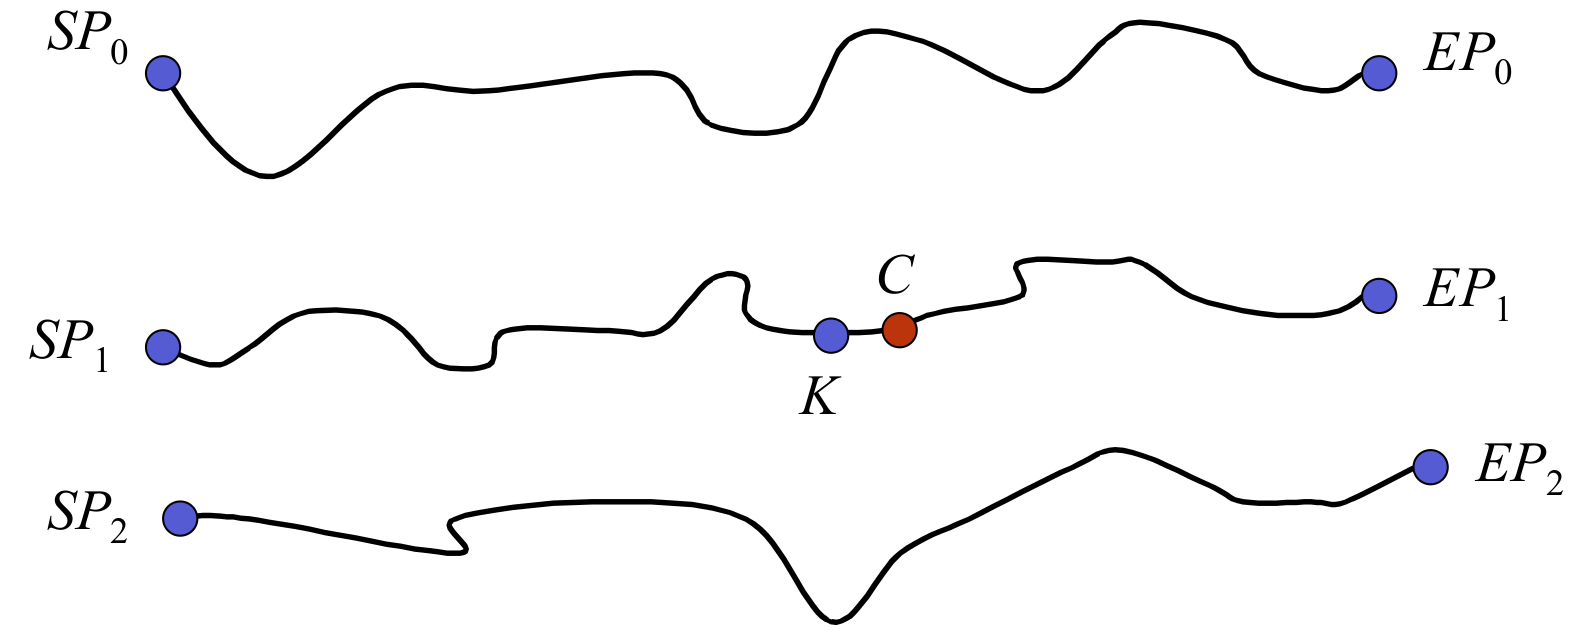
\includegraphics[width=220px]{./chains1.png}
            \end{figure}


            \begin{figure}[h!]
              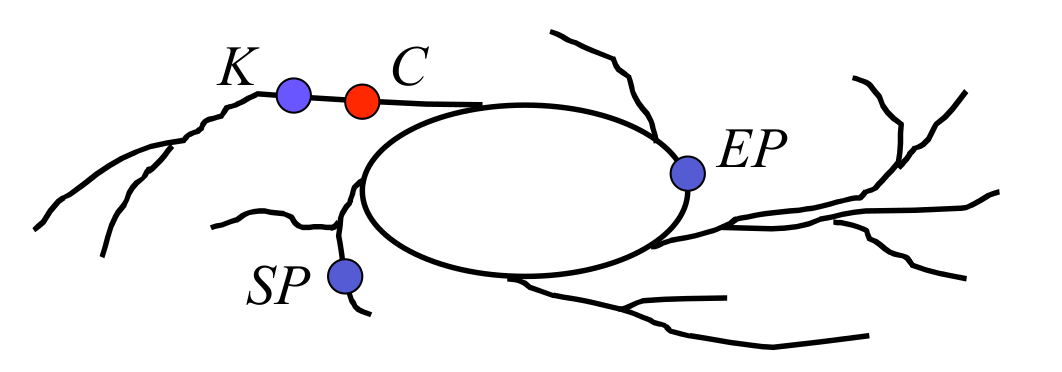
\includegraphics[width=220px]{./chains2.png}
            \end{figure}

        {\bf Rainbow Tables are an improved version of Hellman's algorithm.}
\end{frame}

\begin{frame}
        \frametitle{How Keys are generated anyway?}
        There are three ways keys can be generated:
        \begin{itemize}
          \item By {\bf Randomly} choosing the key from a PRNG,
          \item by {\bf Deriving} the key from a password using a Key Derivation Function,
          \item by using a {\bf Key agreement protocol} that requires
            interactions between involved parties.
        \end{itemize}
\end{frame}